
\begin{figure}
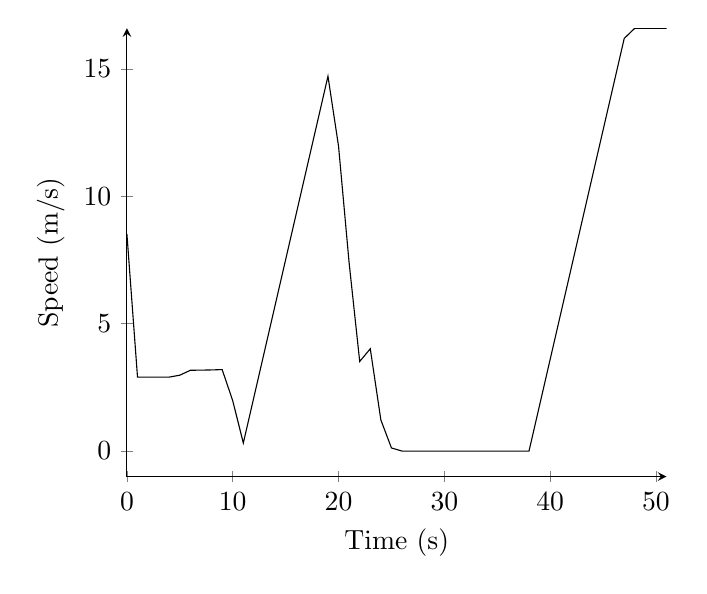
\begin{tikzpicture}
\begin{axis}[
legend style={anchor=west},
axis x line=bottom,
axis y line=left,
ymin=-1,
xlabel=Time (s),
ylabel=Speed (m/s),
]
\addplot[] coordinates {
(0, 8.5161978493)
(1, 2.90367521837)
(2, 2.90369580236)
(3, 2.90372212109)
(4, 2.90375655668)
(5, 2.97928926807)
(6, 3.17230902731)
(7, 3.17747572859)
(8, 3.1855721885)
(9, 3.19951045428)
(10, 1.97570834578)
(11, 0.316915660953)
(12, 2.11691566095)
(13, 3.91691566095)
(14, 5.71691566095)
(15, 7.51691566095)
(16, 9.31691566095)
(17, 11.116915661)
(18, 12.916915661)
(19, 14.716915661)
(20, 11.967652381)
(21, 7.38748309103)
(22, 3.51708497494)
(23, 4.01648075528)
(24, 1.22025745092)
(25, 0.122828451502)
(26, 0.0)
(27, 0.0)
(28, 0.0)
(29, 0.0)
(30, 0.0)
(31, 0.0)
(32, 0.0)
(33, 0.0)
(34, 0.0)
(35, 0.0)
(36, 0.0)
(37, 0.0)
(38, 0.0)
(39, 1.8)
(40, 3.6)
(41, 5.4)
(42, 7.2)
(43, 9.0)
(44, 10.8)
(45, 12.6)
(46, 14.4)
(47, 16.2)
(48, 16.6)
(49, 16.6)
(50, 16.6)
(51, 16.6)
};

\end{axis}
\end{tikzpicture}
\label{tik:speed:100:74}
\caption{100 percent diving with GSC on route $74$}
\end{figure}
